\documentclass[../../project.tex]{subfiles}
\graphicspath{{\subfix{images/}}}

\begin{document}
	The given dataset was bootstrapped 400 times and both DA models were tested before and after input transformations and dropping 'Year' and 'Gross'.
%%	\begin{table}[h!]
%%		\centering
%%		\begin{tabular}{cccc}
%%			Input & DA Model & Mean Accuracy & Mean AUC \\
%%			\midrule
%%			Before transformations
%%			& LDA & 0.856 & 0.870 \\
%%		    & QDA & 0.818 & 0.849 \\
%%			\midrule
%%			After transformations
%%			& LDA & 0.893 & 0.913 \\
%%			& QDA & 0.933 & 0.966 \\
%%		\end{tabular}
%%		\caption{Mean Accuracy and Mean AUC for discriminant analysis models. %%70\% training data.}
%%		\label{tab:discanal_table_70old}
%%	\end{table}
	\begin{table}[h!]
		\centering
		\begin{tabular}{cccc}
			Input & DA Model & Accuracy & AUC \\
			\midrule
			Before transformations
			& LDA & 0.856 & 0.870 \\
		    & QDA & 0.818 & 0.849 \\
			\midrule
			After transformations
			& LDA & 0.900 & 0.917 \\
			& QDA & 0.945 & 0.984 \\
		\end{tabular}
		\caption{Accuracy and AUC for discriminant analysis models using bootstrap. 70\% training data.}
		\label{tab:discanal_table_70}
	\end{table}
%%	\begin{table}[h!]
%%		\centering
%%		\begin{tabular}{cccc}
%%			Input & DA Model & Mean Accuracy & Mean AUC \\
%%			\midrule
%%			Before transformations
%%			& LDA & 0.866 & 0.877 \\
%%		    & QDA & 0.840 & 0.869 \\
%%			\midrule
%%			After transformations
%%			& LDA & 0.903 & 0.915 \\
%%			& QDA & 0.942 & 0.977 \\
%%		\end{tabular}
%%		\caption{Mean Accuracy and Mean AUC for discriminant analysis models. %%90\% training data.}
%%		\label{tab:discanal_table_90old}
%%	\end{table}
		\begin{table}[h!]
		\centering
		\begin{tabular}{cccc}
			Input & DA Model & Accuracy & AUC \\
			\midrule
			Before transformations
			& LDA & 0.866 & 0.877 \\
		    & QDA & 0.840 & 0.869 \\
			\midrule
			After transformations
			& LDA & 0.900 & 0.918 \\
			& QDA & 0.947 & 0.984 \\
		\end{tabular}
		\caption{Accuracy and AUC for discriminant analysis models using bootstrap. 90\% training data.}
		\label{tab:discanal_table_90}
	\end{table}
	From the Tables \ref{tab:discanal_table_70} and \ref{tab:discanal_table_90} we conclude that QDA seems to be more apt for this problem for the final inputs. It is unclear which method performs better for the original inputs. For QDA on the original inputs, the variance in accuracy is high which can be explained by the fact that the original inputs are close to being colinear. This in turn makes $\Sigma$ close to being singular resulting in inaccurate matrix inversion. For example, the standard deviation of accuracy and AUC of the QDA classifier, on the original inputs, with 400 bootstrapped datasets and 90\% training data were 0.076 and 0.081 respectively, compared to 0.021 and 0.019 with the final inputs, ceteris paribus. Fortunately, the final inputs are not colinear.
	
	Cross validation was carried out to estimate the accuracy using 20 folds resulting in an estimated accuracy of 0.949 using 70\% training data. As can be seen in Figure \ref{fig:boxplotQDA}, there is a noticeable variance in accuracy for the different training sets suggesting that there might be outliers in the data that the model has problems accounting for. Increasing the number of folds also increases the minimum accuracy that can be found in the corresponding box-plot, as to be expected. Also using cross validation to compare the effects of input transformations we see a 0.090 increase in accuracy using the final inputs compared to the original inputs. Adding the variables 'Years' and 'Gross' back into the inputs we see a small decrease in accuracy hence they are left out.
	\begin{figure}[ht]
		\centering
    	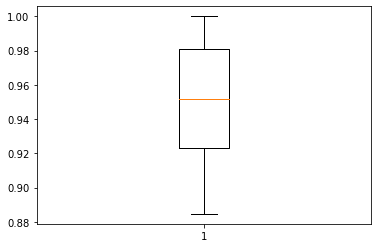
\includegraphics[scale=0.7]{project/tex/QDAboxplot.png}
		\caption{Accuracy estimation using cross validation with 20 folds.}
		\label{fig:boxplotQDA}
    \end{figure}
    
%%   \begin{table}[h!]
%%		\centering
%%		\begin{tabular}{cccc}
%%			Lead & Female & Male \\
%%			\midrule
%%			Female & 75 & 11 \\
%%		    Male & 9 & 217 \\
%%			\midrule
%%		\end{tabular}
%%		\caption{Confusion matrix for QDA. 70\% training data.}
%%		\label{tab:confusionQDA}
%%	\end{table}
\end{document}